\section{Évaluation de la qualité des solutions renvoyées par l'approche génétique}

\subsection{Méthode d'évaluation de la qualité}

Cet algorithme prend en entrée le chemin d'accès vers un répertoire contenant des fichiers \textit{.fjs}. Pour chacun des fichiers présents dans ce répertoire, l'algorithme génétique sera exécuté cinq fois avec les mêmes paramètres. Il s'agira ensuite de calculer le temps moyen des solutions (leur fonction objective), mais aussi le temps d'exécution moyen pour chaque fichier.

Le code correspondant est disponible dans le fichier \textit{evaluatesolutions.py}.

\subsection{Résultats obtenus}

Nous avons décidé de confronter notre algorithme aux résultats connus pour le \textit{Brandimarte\_Data}. Dans les tableaux suivants, LB correspond aux bornes inférieures connues et UB aux bornes supérieures connues de l'optimum. $n$ correspond au nombre de job et $m$ au nombre de machines.

Les temps moyens d'exécution sont donnés en secondes.

\subsubsection{Résultats de notre algorithme pour une population de 50 individus et une génération maximale de 150}

\begin{table}[!h]
    \renewcommand{\arraystretch}{1.5}
    \centering
    \begin{tabular}{p{\textwidth/7} c c c c c}
        Instance & $n \times m$ & LB & UB & Temps moyen & Temps d'exécution moyen \\
         \hline
        Mk01 & $10 \times 6$ & \textbf{40} & \textbf{40} & 44.4 & 6.91 \\
         \hline
        Mk02 & $10 \times 6$ & \textbf{26} & \textbf{26} & 40.8 & 11.1 \\
         \hline
        Mk03 & $15 \times 8$ & \textbf{204} & \textbf{204} & 235.6 & 22.6 \\
         \hline
        Mk04 & $15 \times 8$ & \textbf{60} & \textbf{60} & 72.8 & 10.71 \\
         \hline
        Mk05 & $15 \times 4$ & \textbf{172} & \textbf{172} & 189 & 12.02 \\
         \hline
        Mk06 & $10 \times 15$ & \textbf{57} & \textbf{57} & 114.2 & 26.73 \\
         \hline
        Mk07 & $20 \times 5$ & \textbf{139} & \textbf{139} & 198 & 15.45 \\
         \hline
        Mk08 & $20 \times 10$ & \textbf{523} & \textbf{523} & 523 & 22.13 \\
         \hline
        Mk09 & $20 \times 10$ & \textbf{307} & \textbf{307} & 391.4 & 34.11 \\
         \hline
        Mk10 & $20 \times 15$ & 189 & 193 & 317 & 39.95 \\
         \hline 
    \end{tabular}
\end{table}

\begin{figure}[!h]
    \centering
    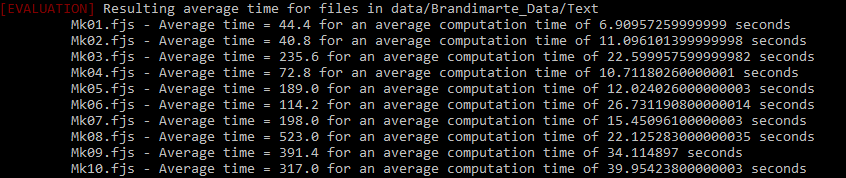
\includegraphics[width=\linewidth]{report/Pictures/brandimarte_50_150.png}
\end{figure}

\subsubsection{Résultats de notre algorithme pour une population de 200 individus et une génération maximale de 500}

\begin{table}[!h]
    \renewcommand{\arraystretch}{1.5}
    \centering
    \begin{tabular}{p{\textwidth/7} c c c c c}
        Instance & $n \times m$ & LB & UB & Temps moyen & Temps d'exécution moyen \\
         \hline
        Mk01 & $10 \times 6$ & \textbf{40} & \textbf{40} & 42.4 & 108.91 \\
         \hline
        Mk02 & $10 \times 6$ & \textbf{26} & \textbf{26} & 34.4 & 202.02 \\
         \hline
        Mk03 & $15 \times 8$ & \textbf{204} & \textbf{204} & 207.4 & 359.07 \\
         \hline
        Mk04 & $15 \times 8$ & \textbf{60} & \textbf{60} & 69 & 166.65 \\
         \hline
        Mk05 & $15 \times 4$ & \textbf{172} & \textbf{172} & 179.4 & 176.70 \\
         \hline
        Mk06 & $10 \times 15$ & \textbf{57} & \textbf{57} & 96.2 & 439.49 \\
         \hline
        Mk07 & $20 \times 5$ & \textbf{139} & \textbf{139} & 169.2 & 225.43 \\
         \hline
        Mk08 & $20 \times 10$ & \textbf{523} & \textbf{523} & 523 & 353.90 \\
         \hline
        Mk09 & $20 \times 10$ & \textbf{307} & \textbf{307} & 351.4 & 528.68 \\
         \hline
        Mk10 & $20 \times 15$ & 189 & 193 & 282.8 & 568.81 \\
         \hline 
    \end{tabular}
\end{table}

\begin{figure}[!h]
    \centering
    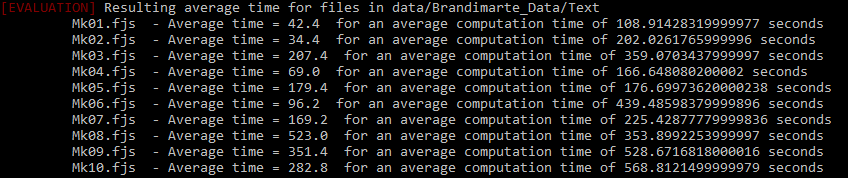
\includegraphics[width=\linewidth]{report/Pictures/brandimarte_200_500.png}
\end{figure}

\newpage

\subsubsection{Résultats de notre algorithme pour une population de 500 individus et une génération maximale de 1000}

\begin{table}[!h]
    \renewcommand{\arraystretch}{1.5}
    \centering
    \begin{tabular}{p{\textwidth/7} c c c c c}
        Instance & $n \times m$ & LB & UB & Temps moyen & Temps d'exécution moyen \\
         \hline
        Mk01 & $10 \times 6$ & \textbf{40} & \textbf{40} & 41.6 & 521.59 \\
         \hline
        Mk02 & $10 \times 6$ & \textbf{26} & \textbf{26} & 31.2 & 928.05 \\
         \hline
        Mk03 & $15 \times 8$ & \textbf{204} & \textbf{204} & 204 & 1880.24 \\
         \hline
        Mk04 & $15 \times 8$ & \textbf{60} & \textbf{60} & 67 & 879.17 \\
         \hline
        Mk05 & $15 \times 4$ & \textbf{172} & \textbf{172} & 178.6 & 959.05 \\
         \hline
        Mk06 & $10 \times 15$ & \textbf{57} & \textbf{57} & 82.2 & 1845.56 \\
         \hline
        Mk07 & $20 \times 5$ & \textbf{139} & \textbf{139} & 155.2 & 1181.74 \\
         \hline
        Mk08 & $20 \times 10$ & \textbf{523} & \textbf{523} & 523 & 1978.39 \\
         \hline
        Mk09 & $20 \times 10$ & \textbf{307} & \textbf{307} & 339 & 2680.10 \\
         \hline
        Mk10 & $20 \times 15$ & 189 & 193 & 263.6 & 3228.08 \\
         \hline 
    \end{tabular}
\end{table}

\begin{figure}[!h]
    \centering
    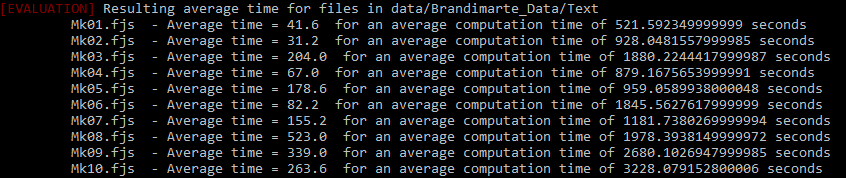
\includegraphics[width=\linewidth]{report/Pictures/brandimarte_500_1000.png}
\end{figure}

\subsubsection{Interpolation des résultats et temps de calcul nécessaire pour arriver à l'optimum}

Supposons que la meilleure solution trouvée soit fonction du temps de calcul. En effet, plus l'algorithme génétique tourne longtemps, plus il a de chance de converger vers l'optimum.

Nous ne nous intéresserons pas aux fichiers \textit{Mk03} et \textit{Mk08} car les solutions optimales ont été trouvées précédemment, ni à \textit{Mk10} car l'optimum n'est pas connu.

\begin{figure}[!h]
    \centering
    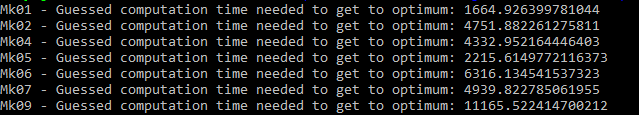
\includegraphics[width=\linewidth]{report/Pictures/guessed_computation_time_brandimarte.png}
\end{figure}

En relançant un certain nombre d'instance de l'algorithme génétique, nous sommes parvenu à interpoler les fonctions objectives en fonction du temps de calcul pour chaque fichier à l'aide d'un algorithme appelé \textit{Piecewise Cubic Hermite Interpolating Polynomial} dont nous ne rentrerons pas dans les détails techniques. A partir de ces interpolations, nous cherchons pour quel temps de calcul nous obtenons la fonction objective optimale.

\begin{figure}[!h]
    \centering
    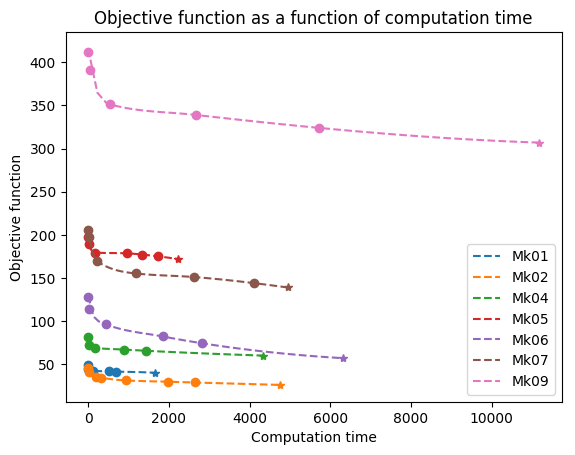
\includegraphics[width=\linewidth]{report/Pictures/objective_function_as_function_of_time.png}
\end{figure}

Les ronds correspondent aux points résultant des évaluations de l'algorithme génétique, les étoiles aux optima connus et les courbes en pointillé correspondent aux splines résultant des interpolations.

Ces résultats sont cependant à prendre avec des pincettes, absolument rien ne les garantie principalement du fait du peu de nombres de points que l'on a calculé (il nous a fallu plusieurs jours pour calculer cet ensemble de points étant donné que l'on a repris le principe d'évaluation des solutions décrit précédemment, la contrainte temporelle nous a donc limité sur la densité de cet ensemble).

\newpage